\documentclass{article}
\usepackage{xeCJK,amsmath,geometry,graphicx,amssymb,zhnumber,booktabs,setspace,tasks,verbatim,amsthm,amsfonts,mathdots}
\usepackage{listings,xcolor,float,caption,subfigure}
\geometry{a4paper,scale=0.8}   
\renewcommand\arraystretch{2}
\title{ICS  HomeWork-3}
\author{PB20000113孔浩宇}
\begin{document}
\maketitle
\section*{T1}如图
    \begin{table}[!ht]
        \centering
        \begin{tabular}{|c|c|c|c|c|c|}
        \hline
            $S1$ & $S0$ & $X$ & $Z$ & $S1'$ & $S0'$ \\ \hline
            0 & 0 & 0 & 1 & 0 & 0  \\ \hline
            0 & 0 & 1 & 1 & 0 & 1  \\ \hline
            0 & 1 & 0 & 0 & 1 & 0  \\ \hline
            0 & 1 & 1 & 0 & 0 & 0  \\ \hline
            1 & 0 & 0 & 0 & 0 & 1  \\ \hline
            1 & 0 & 1 & 0 & 1 & 0  \\ \hline
            1 & 1 & 0 & 0 & 0 & 0  \\ \hline
            1 & 1 & 1 & 0 & 0 & 0  \\ \hline
        \end{tabular}
    \end{table}
    \begin{figure*}[htbp]
        \centering
        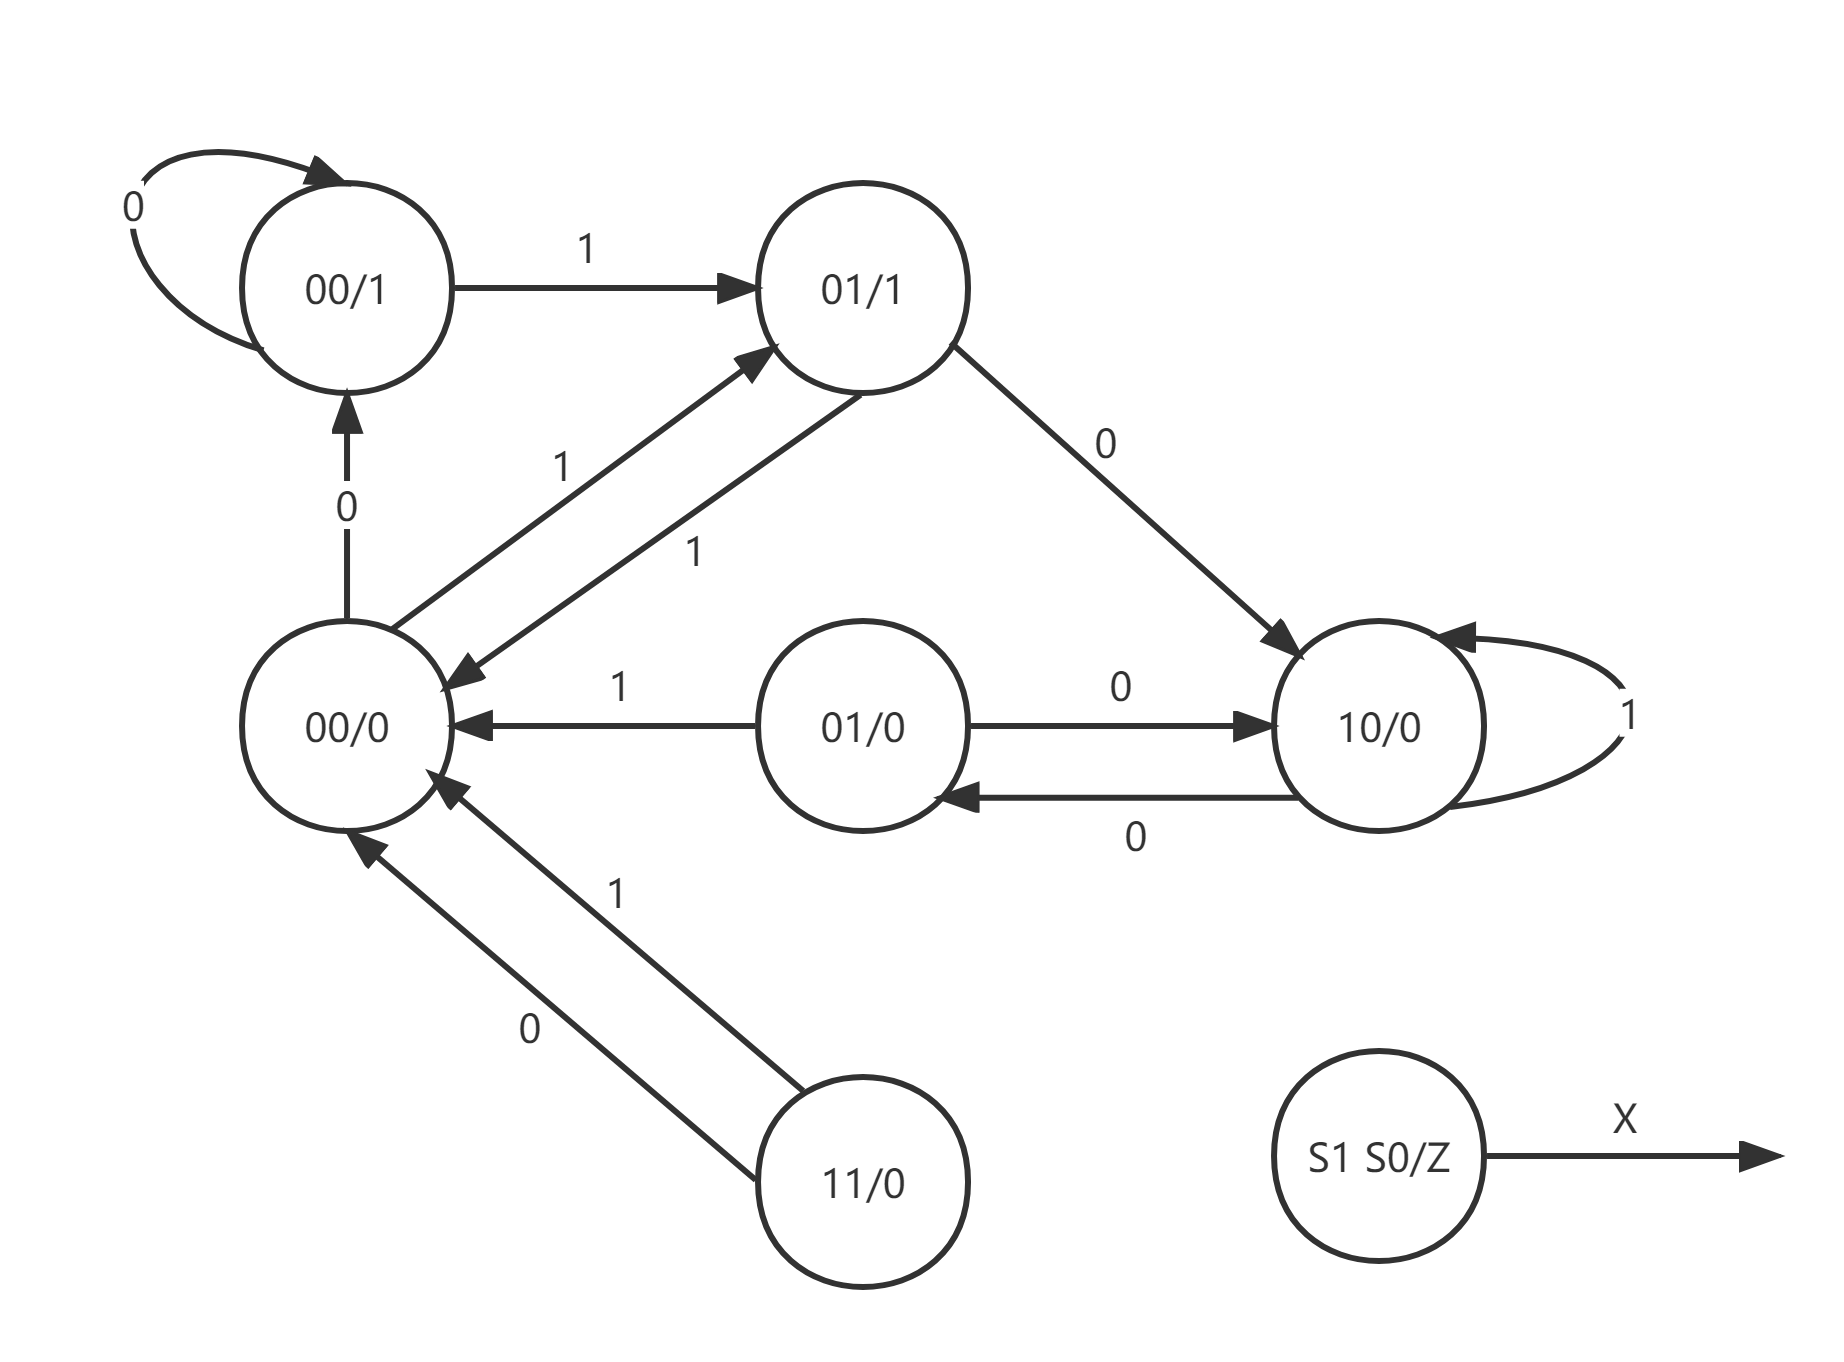
\includegraphics[scale=0.15]{T1.png}
    \end{figure*}
\section*{T2}
    如果$R_1+R_2 \geq 0$,则下条指令执行$x3039$.
\section*{T3}
\begin{enumerate}
    \item [(a)]$Bits[15:12]$表示指令的操作码,即指令做什么
    \item [(b)]$Bits[11:0]$表示操作数,即指令对谁操作
\end{enumerate}
\section*{T4}
    \begin{enumerate}
        \item [(1)] 取指令:需要读取内存中数据,即$MDR <- M[MAR]$,需100个时钟周期。
        
        \item [(2)] 译码:从IR寄存器中读$IR[15:12]$,需要1个时钟周期
            
        \item [(3)] 地址计算:不需要进行
    
        \item [(4)] 取操作数:从IR寄存器中读取,需1个时钟周期
        
        \item [(5)] 执行:需1个时钟周期
        
        \item [(6)] 存放结果:将结果写入寄存器$R_6$,需要1个时钟周期
    \end{enumerate}
    共需100+1+1+1+1=104个周期。
\section*{T5}
    操作数需要6位来表示,寄存器地址需要6位,则立即数至多为14位,表示范围为$-2^{13} \sim 2^{13}-1$.
\section*{T6}
    \begin{enumerate}
        \item [(a)]对$1001 (NOT)$没有好处;对$0001,0101$可以增加立即数表示位数,扩大立即数表示范围.
        \item [(b)]对$0010 (LD),0011 (ST)$,偏移量位数增加,可寻址范围增加.
        \item [(c)]对$0000 (BR)$没有好处.
    \end{enumerate}
\section*{T7}
    \begin{table}[!ht]
        \centering
        \begin{tabular}{|c|c|c|c|c|c|c|}
        \hline
            ~ & fetch instruction & decode & evaluate address & fetch data & execute & store result  \\ \hline
            PC & All & ~ & ~ & ~ & JMP &   \\ \hline
            IR & All & ~ & ~ & ~ & ~ &   \\ \hline
            MAR & All & ~ & STR & All & ~ &   \\ \hline
            MDR & All & ~ & STR & All & ~ &   \\ \hline
        \end{tabular}
    \end{table}
\section*{T8}如图
\begin{figure}[htbp]
    \centering
    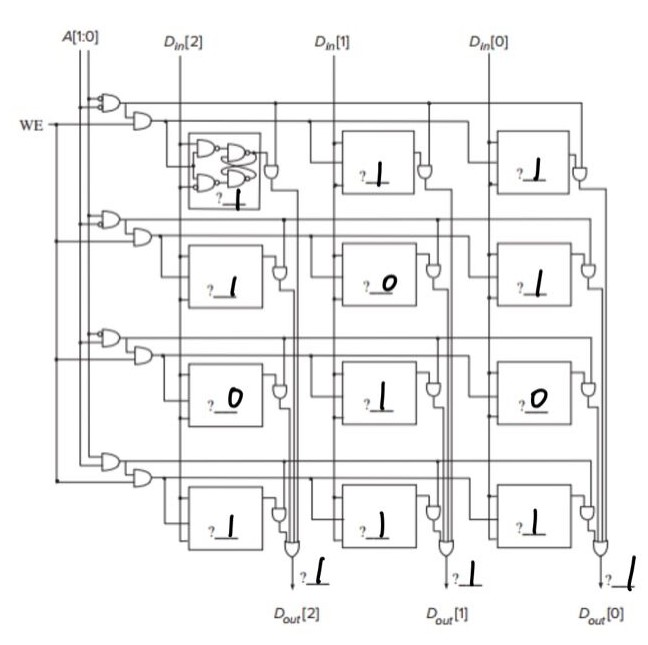
\includegraphics[scale=0.8]{t8.jpg}
\end{figure}
\section*{T9}
\begin{enumerate}
    \item [(a)]$MAR:x2 \qquad MDR:01010000$
    \item [(b)]$MDR: 00111001$
\end{enumerate}
\section*{T10}
    \begin{table}[!ht]
        \centering
        \begin{tabular}{|c|c|c|c|}
        \hline
            ~ & R/W & MAR & MDR  \\ \hline
            Operation 1 & W & x4000 & 1 1 1 1 0  \\ \hline
            Operation 2 & R & x4003 & 1 0 1 1 0  \\ \hline
            Operation 3 & W & x4001 & 1 0 1 1 0  \\ \hline
            Operation 4 & R & x4002 & 0 1 1 0 1  \\ \hline
            Operation 5 & W & x4003 & 0 1 1 0 1  \\ \hline
        \end{tabular}
    \end{table}
\section*{T11}
\begin{enumerate}
    \item [(a)]至少需要8位来表示操作码
    \item [(b)]至少需要7位来表示寄存器
    \item [(c)]最大位数为3位
\end{enumerate}
\section*{T12}
\begin{enumerate}
    \item [(a)]每秒产生的机器周期数为
    \[
        n=\displaystyle{\frac{1}{T}}
        =\displaystyle{\frac{1}{2\times 10^{-9}}}
        =5\times 10^{8}.
    \]
    \item [(b)]每秒处理的指令最多为
    \[
        n=\displaystyle{\frac{5\times 10^{8}}{8}}
        =6.25\times 10^{7}.
    \]
    \item [(c)]每秒能执行指令
    \[
        n=6\times 6.25\times 10^{7}
        =3.75\times 10^{8}.
    \]
\end{enumerate}

\section*{T13}
\begin{enumerate}
    \item [(1)] 取指令:将当前PC装入MAR,PC增量;将地址MAR对应的数据$M[MAR]$写入MDR,并将MDR的内容写入IR寄存器。
    
    \item [(2)] 译码:通过IR寄存器中的前四位来判断该指令是什么操作。
        
    \item [(3)] 地址计算:如果涉及地址的计算,在这一拍进行。

    \item [(4)] 取操作数:从IR中读取该指令操作的对象。
    
    \item [(5)] 执行:对操作数执行该指令对应的操作。
    
    \item [(6)] 存放结果:将结果写入最后结果对应的寄存器。
\end{enumerate}
\end{document}
 